\documentclass[12pt,a4paper]{article}
\usepackage[UTF8]{ctex}
\usepackage{amsmath,amssymb}
\usepackage{booktabs}
\usepackage{multirow}
\usepackage{siunitx}
\usepackage{float}
\usepackage{fancyhdr}   % 页眉页脚控制
\usepackage{geometry}
\usepackage{subfigure}  % 子图排版
\usepackage{subcaption}
\usepackage{graphicx}
\usepackage{listings} % 代码排版宏包
\usepackage{xcolor} % 代码高亮颜色
\usepackage{enumitem} % 列表格式控制宏包
\geometry{left=2.5cm,right=2.5cm,top=2.5cm,bottom=2.5cm}

\pagestyle{fancy}
\fancyhf{} % 清空默认页眉页脚
\fancyhead[L]{\small 长度密度测量}       % 左上角页眉
\fancyhead[R]{\small 2513318}          % 右上角章节名
\fancyfoot[C]{\thepage}                   % 居中页码（页脚）
\renewcommand{\headrulewidth}{0.4pt}      % 页眉线粗细
\renewcommand{\footrulewidth}{0.4pt}      % 页脚线粗细
%报告开始
\begin{document}
	%设置课程标题
	\begin{center}
		\heiti\LARGE{《大学基础物理实验》课程实验报告}
	\end{center}
	%设置实验人信息以及实验时间表格
	\begin{center}
		\begin{tabular}{lcr}
			{\songti 姓名及学号：陈秋实2513318}  \quad 专业：密码科学与技术 \quad 组别：L组1号 \\
			{\songti  学院：密码与网络空间安全学院 \quad 实验时间：2026年6月12日~星期五~下午}\\
		\end{tabular}
	\end{center}
	\vspace{-0.2cm}
	{\noindent}	 \rule[-10pt]{16cm}{0.05em}\\
	\vspace{-0.4cm}

	%实验题目
	\begin{center}
		\LARGE\textbf{长度密度测量}
	\end{center}
	
	
	\section{实验目的}
	\par 1.了解米尺、游标卡尺、螺旋测微器的测量原理和使用方法；
	\par 2.掌握用流体静力称衡法测定不规则固体密度的原理和方法；
	\par 3.熟悉仪器的读数规则及有效数字运算法则；
	\par 4.掌握直接测量、间接测量的数据处理方法及测量不确定度估计方法。

	
	\section{实验器材}
	\par 米尺，游标卡尺，螺旋测微器，钢球，空心柱体，牛角扣，电子天平，铁架台，玻璃烧杯，细线，温度计等
	
	\section{实验原理}
	\par 1.\textbf{读数问题}
	\[
	\text{50分度游标卡尺：}12.81cm\to 12.810cm \quad 
	\text{螺旋测微器：}7.564cm  \to 7.5642cm\\
	\]
	\par 2.\textbf{米尺} 量程0-1000.0mm，分度值1.0mm 估读到0.00cm；
	\par 3.\textbf{游标卡尺}
	\begin{figure}[!htbp]
		\centering
		\includegraphics*[width=0.7\textwidth]{游标卡尺.png}
	\end{figure}
	游标卡尺 50格的仪器，读数到00.00mm；游标卡尺是在米尺上附加一个刻度均匀且可以滑动的游标，从而巧妙地提高米尺的测量精度。游标卡尺的结构如图所示，量爪A、C与主尺L相连，B、D及深度尺G与副尺S相连；M为紧固螺钉，N为推把。A、B组成内测量爪，可测内径及槽宽；C、D组成外测量爪，可测长度、厚度及外径；G可测深度及台高。当卡口合拢时，主、副尺“0”刻度线重合，深度尺端面与主尺端面重合。主尺的长度决定了游标卡尺的量程，副尺的刻度决定了游标卡尺的分度值。
	\par 游标卡尺的主尺上$n-1$个分度所对应的长度为$(n-1)mm$；副尺上$n$个分度所对应的长度也是$(n-1)mm$，如下图所示，因此主尺与刚尺每个分度简之差即格差为
	\[
	\varepsilon_{x}=(1-{\frac{n-1}{n}})m m={\frac{1}{n}}m m
	\]
	\par $\varepsilon_{x}$就是游标卡尺的最小分划单位即分度值。由于$\varepsilon_{x}$可由格差精确地给出，所以卡尺的测量精度明显优于米尺，我们所使用的50分度游标卡尺所对应的分度值分别为$0.02mm$。
	游标卡尺的读数方法是：游标卡尺的读数由主尺读数和副尺读数两部分组成，主尺上读出毫米位的准确数，毫米以下的尾数由副尺读出。若副尺上第m个刻线与主尺上某刻线$(k+m)$重合，因格差为$\varepsilon_{x}$，故可断定副尺零刻线与主尺上第$k$个刻度线相距$m\varepsilon_{x}$。于是可得待测长度为
	\[
	x=k\;m m+m\varepsilon_{x}
	\]
	\par 用游标卡尺的不同测量爪分别测量半空心圆柱体的外径$D_1$、内径$D_2$、高度$H_1$及深度$H_2$,再利用公式
	\[
	V={\frac{\pi}{4}}(D_{1}^{2}H_{1}-D_{2}^{2}H_{2})
	\]
	可以求出半空心圆柱体的体积。
	\par 4.\textbf{螺旋测微器}
	\par 量程为25mm，分度值为0.01mm，估读到0.000mm；螺旋测微器是利用螺旋进退来测量长度的仪器，它比游标卡尺更精密，常用于测量小球的直径、金属丝的直径和薄板的厚度。实验室中常用的螺旋测微器量程为25mm，分度值为0.01mm，极限误差为0.004mm。
	\begin{figure}[!htbp]
		\centering
		\includegraphics*[width=0.5\textwidth]{螺旋测微器.png}
	\end{figure}
	\par 测微螺杆和微分筒（副尺）、棘轮相连，并以螺纹与固定套管（主尺）连接。轻转棘轮，则棘轮靠一定的摩擦力带动副尺一起转动;当微分筒相对于固定套管转过一周时，测微螺杆前进或者后退一个螺距。主尺分度为$0.5mm$，螺纹的螺距为$0.5mm$，因此副尺旋转一周，即在主尺上移动一格，即顶砧A与测微螺杆B端面的间距改变$0.5mm$。副尺套筒上均分$50$个小格，因此，每旋转1小格测杆B移动$0.5/50mm=0.01mm$。可见，螺旋测微器的设计特点就是采用了这种机械放大原理。读数时，要读出主尺上的读数还有微分筒上的读数，注意不要丢掉主尺上可能露出的“半整数”，副尺读数时应包括一位小数。此外，使用螺旋测微器测量物体之前，应先记录零点读数$x_0$。这是因为当转动棘轮使测微螺杆与顶砧刚接触时，微分筒的端面的读数应为$0.000mm$，否则就应该记录初始读数，也就是零点读数，以便对测量值进行修正，测量结果应是:测量值=读数值-零点读数。读零点读数时应注意微分筒上的零刻度线在主尺横线的上方还是下方，对应零点读数分别为正值还是负值。测量得到小刚球的直径$D$后根据以下公式计算体积
	\[
	V_{\text{球}}=\frac{4}{3}{\pi}(\frac{D}{2})^{3}=\frac{{\pi}D^{3}}{6}
	\]
	\par 5.\textbf{流体静力称衡法}
	\par 若物体质量为$m$,体积为$V$，则其密度为
	\[
	\rho = \frac{m}{V}
	\]
	\par 由阿基米德原理：物体在液体中所受的浮力等于它排开液体的重量。若以$\rho_0$表示液体的密度，$V$表示排开液体的体积亦即待测物体的体积。进行受力分析如下
	\begin{figure}[!htbp]
		\centering
		\begin{minipage}[t]{0.4\textwidth}
			\centering
			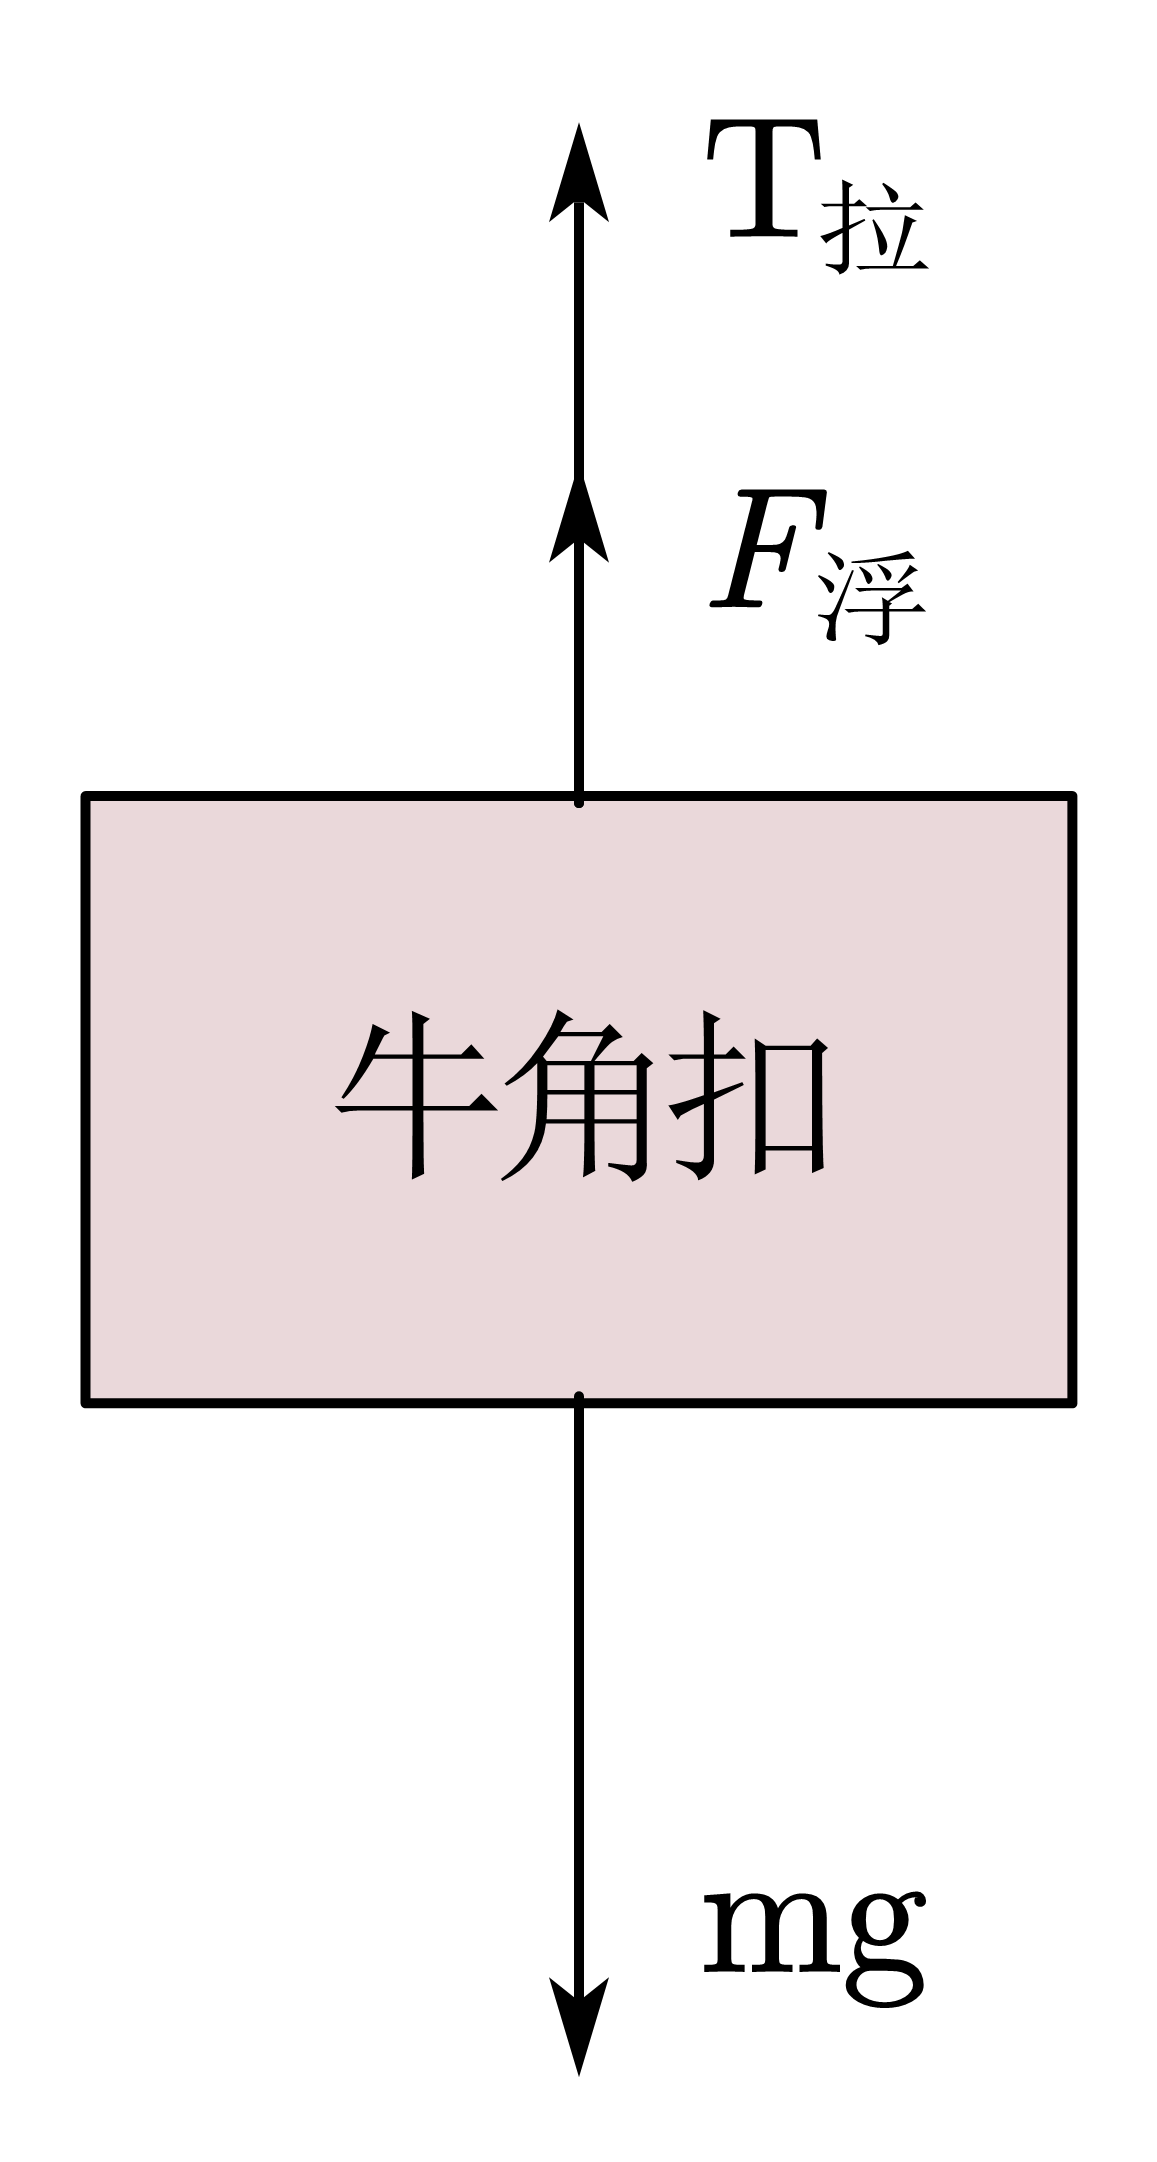
\includegraphics[width=3.5cm]{牛角扣受力分析.png}
			\caption{牛角扣受力分析}
		\end{minipage}
		\begin{minipage}[t]{0.4\textwidth}
			\centering
			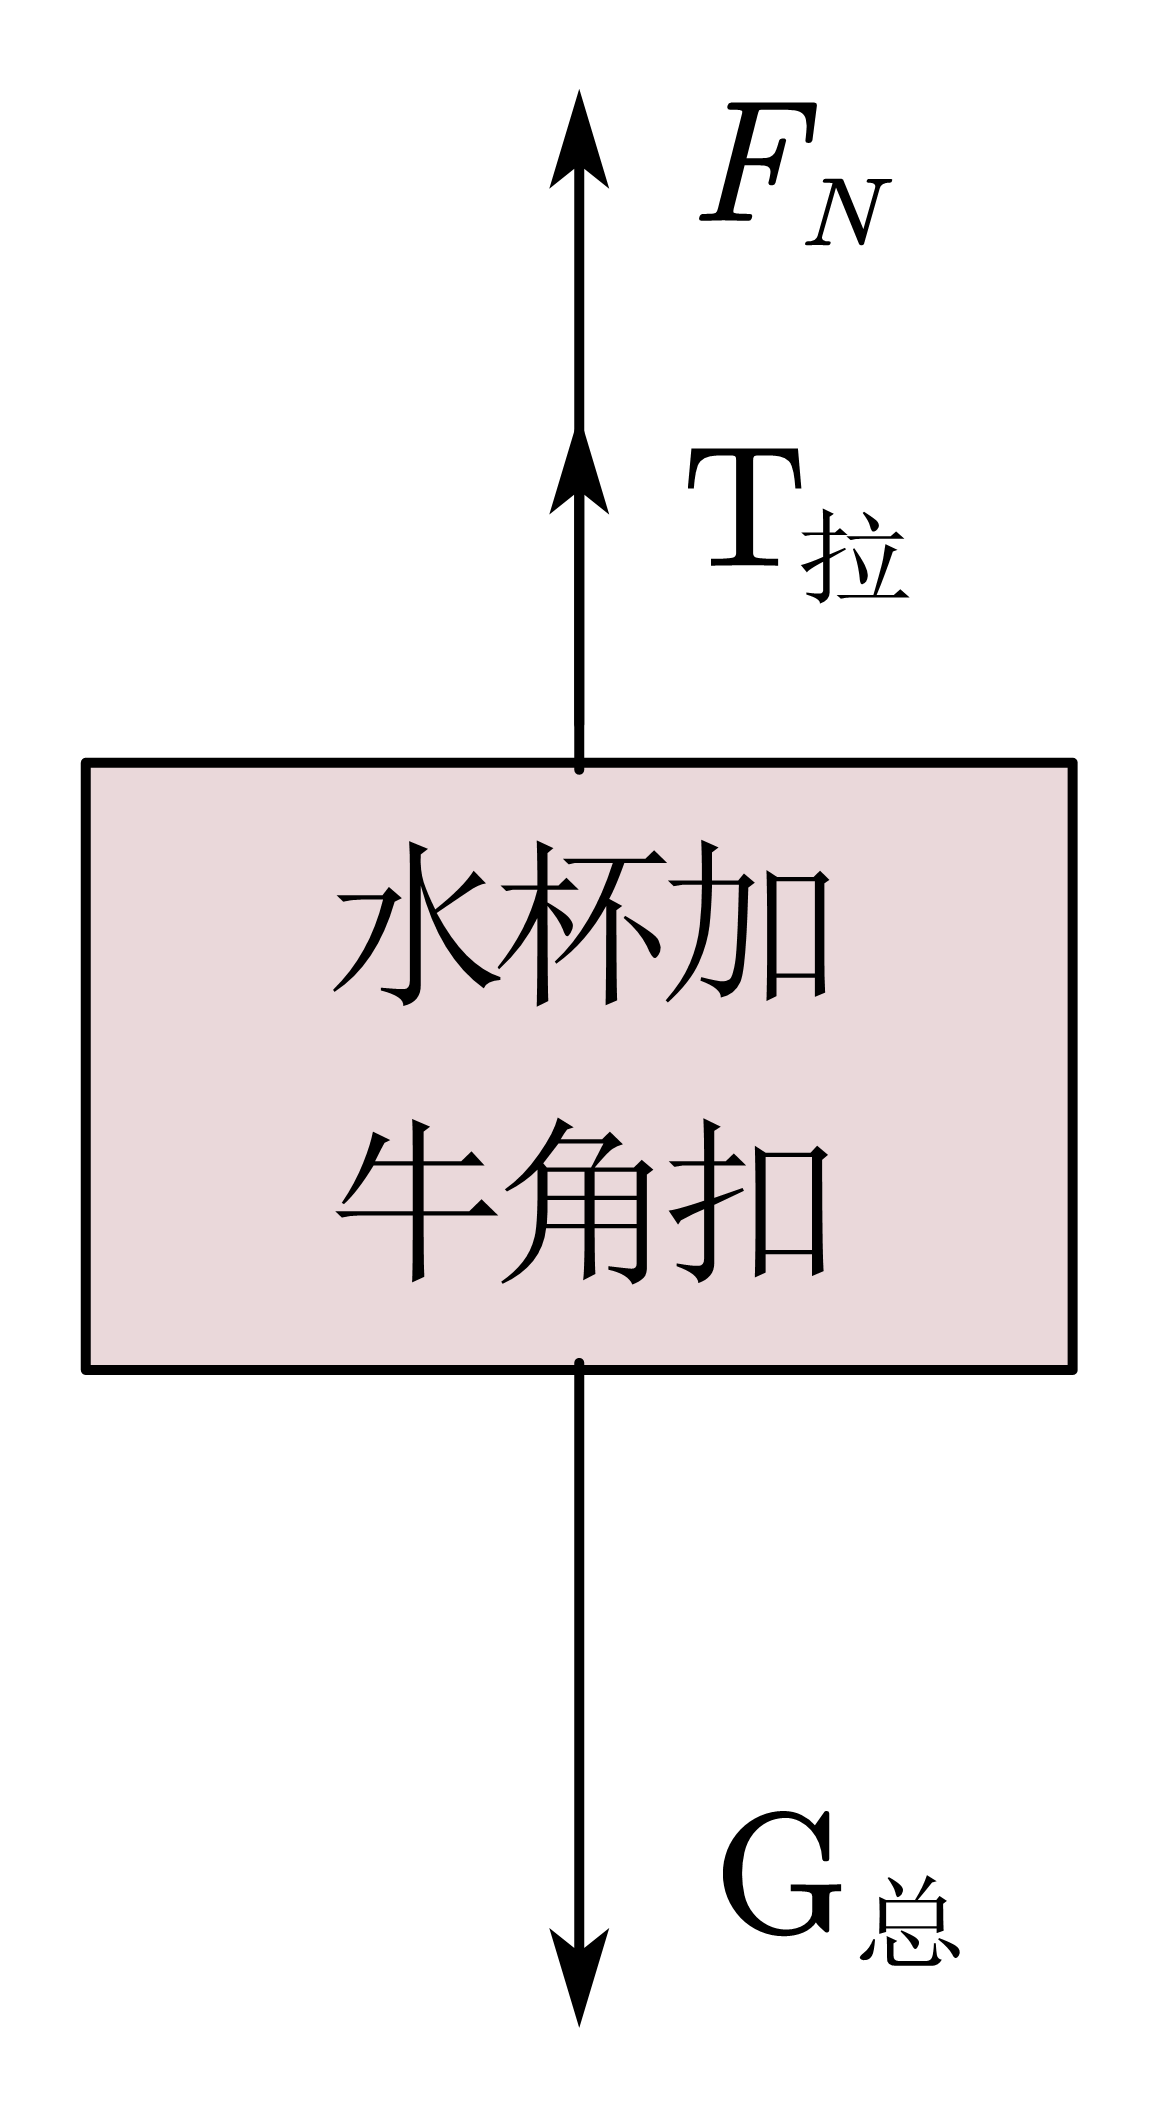
\includegraphics[width=3.5cm]{水和烧杯受力分析.png}
			\caption{整体受力分析}
		\end{minipage}
	\end{figure}
	\par 由图可知，牛角扣受力分析方程如下：
	\begin{align*}
		\left\{
		\begin{aligned}
			T_{\text{拉}}+F_{\text{浮}}&=mg\\
			T_{\text{拉}}+F_{N}&=G_{\text{总}}
		\end{aligned}
		\right.
	\end{align*}
	\par 其中$G_{\text{总}}$为表格中的$(m_0+m)g$,$F_N$为表格中的$m_1g$，两式消去$T_{\text{拉}}$后得到
	\[
	F_{\text{浮}} = (m_1-m_0)g
	\]
	\par 由阿基米德原理:
	\[
	F_{\text{浮}} = \rho_0 V g
	\]
	\par 查表得到$\rho$，由此解出$V$，带入密度表达式，解出
	\[
	\rho = \frac{m \rho_o}{m_1-m_0}
	\]
	
	
	\section{实验内容}
	\begin{enumerate}
		\item 用米尺测教科书宽度$l$：测量时采取四种不同的方法各测$4$次。
		\begin{itemize}
			\item[(1)] 米尺同一起点，测量教科书同一位置，测得$l_1$；
			\item[(2)] 同一起点，不同位置，测得$l_2$；
			\item[(3)] 不同起点，同一位置，测得$l_3$；
			\item[(4)] 不同起点，不同位置，测得$l_4$。
		\end{itemize}
		\item 用游标卡尺在不同方位测半空心圆柱体的外径$D_1$，内径$D_2$，高$H_1$，深$H_2$各$4$次，并计算其体积；
		\item 用螺旋测微器测小钢球的直径$D$ $6$次，并计算其体积；
		
		\item 用流体静力称衡法测定牛角扣的密度（不要求不确定度）。
		\begin{itemize}
			\item[(1)] 用电子天平称量牛角扣的质量（$m$）$1$次；
			\item[(2)] 用电子天平称量装满水的烧杯质量（$m_0$），记录；将系有绳子的牛角扣完全浸没在水中，记录电子天平视重（$m_1$）；
			\item[(3)] 把牛角扣拿出并擦干，将烧杯里的水倒出一些，记录此时装水烧杯的质量；再次将牛角扣完全浸没在烧杯里的水中，记录电子天平视重；
			\item[(4)] 再一次擦干牛角扣，倒水，放入牛角扣，记录装水烧杯的质量和浸入牛角扣后的视重。
			\item[(5)] 最终得到$3$组浸入牛角扣前后的视重数据。
		\end{itemize}
	\end{enumerate}
	
	\subsection{数据处理}
	\subsubsection*{教科书的宽度}

    \begin{table}[H]
    	\centering
    	\caption{教科书宽度测量数据记录与处理表（单位：$10^{-2}\,\text{m}$，$\Delta_{\text{仪}}=0.05\,\text{cm}$）}
    	\label{tab:book_width}
    	\footnotesize
    	\resizebox{\textwidth}{!}{%
    	\begin{tabular}{|c|c|c|c|c|c|c|c|c|c|c|c|c|}
    		\hline
    		\multirow{2}{*}{次数} &
    		\multicolumn{2}{c|}{$l_1$} &
    		\multicolumn{2}{c|}{$l_2$} &
    		\multicolumn{4}{c|}{$l_3$} &
    		\multicolumn{4}{c|}{$l_4$} \\
    		\cline{2-13}
    		& $l_1$ & $\nu_{l_1}$ & $l_2$ & $\nu_{l_2}$ & 起点 & 终点 & $l_3$ & $\nu_{l_3}$ & 起点 & 终点 & $l_4$ & $\nu_{l_4}$ \\
    		\hline
    		1 & 17.71 & $+$0.0075 & 17.70 & $-$0.0025 & 3.00 & 20.70 & 17.70 & $-$0.0025 & 3.00 & 20.70 & 17.70 & 0.0000 \\
    		\hline
    		2 & 17.70 & $-$0.0025 & 17.71 & $+$0.0075 & 6.00 & 23.70 & 17.70 & $-$0.0025 & 6.00 & 23.69 & 17.69 & $-$0.0100 \\
    		\hline
    		3 & 17.70 & $-$0.0025 & 17.70 & $-$0.0025 & 9.00 & 26.71 & 17.71 & $+$0.0075 & 9.00 & 26.71 & 17.71 & $+$0.0100 \\
    		\hline
    		4 & 17.70 & $-$0.0025 & 17.70 & $-$0.0025 & 12.00 & 29.70 & 17.70 & $-$0.0025 & 12.00 & 29.70 & 17.70 & 0.0000 \\
    		\hline
    		平均 & 17.725 & $s=$0.0050 & 17.725 & $s=$0.0050 & — & — & 17.725 & $s=$0.0050 & — & — & 17.70 & $s=$0.0082 \\
    		\hline
    		$u_A$ & — & 0.0025 & — & 0.0025 & — & — & — & 0.0025 & — & — & — & 0.0041 \\
    		\hline
    		$u_B$ & — & 0.0289 & — & 0.0289 & — & — & — & 0.0289 & — & — & — & 0.0289 \\
    		\hline
    		$u_x$ & — & \textbf{0.029} & — & \textbf{0.029} & — & — & — & \textbf{0.029} & — & — & — & \textbf{0.029} \\
    		\hline
    	\end{tabular}%
    	}
    \end{table}


	\par 表中 $\nu_{l_i}=l_i-\bar{l}_i$ 为残差。样本标准差按贝塞尔公式计算：
	\[
	s_{l_i}=\sqrt{\frac{\sum_{j=1}^{4}(l_{i_j}-\bar{l}_i)^2}{4-1}},\qquad
	u_A=\frac{s_{l_i}}{\sqrt{n}}=\frac{s_{l_i}}{\sqrt{4}},\qquad
	\]
	\[
	u_B=\frac{\Delta_{\text{仪}}}{\sqrt{3}}=\frac{0.05}{\sqrt{3}}\approx 0.0289\,\text{cm},\qquad
	u_x=\sqrt{u_A^2+u_B^2}
	\]
	
	\par 最终测量结果（单位：$10^{-2}\,\text{m}$）：
	\begin{align*}
		l_1 &= (17.70 \pm 0.03) \times 10^{-2}\,\text{m} \\
		l_2 &= (17.70 \pm 0.03) \times 10^{-2}\,\text{m} \\
		l_3 &= (17.70 \pm 0.03) \times 10^{-2}\,\text{m} \\
		l_4 &= (17.70 \pm 0.03) \times 10^{-2}\,\text{m}
	\end{align*}
	
	
	
	\subsection*{半空心圆柱几何尺寸}
	\begin{table}[H]
		\centering
		\caption{半空心圆柱几何尺寸测量数据记录与处理表（游标卡尺）}
		\label{tab:cylinder_comprehensive}
		\footnotesize
		\makebox[\textwidth][s]{
			单位：(cm)\hfill
			零点读数 $x_0 = 0.000$\hfill
			允差：$\Delta_x = 0.002$%
		}
		\begin{tabular}{|c|c|c|c|c|c|c|c|c|}
			\hline
			次数 & $D_{1i}$ & $S_{D_{1i}}$ & $H_{1i}$ & $S_{H_{1i}}$ & $D_{2i}$ & $S_{D_{2i}}$ & $H_{2i}$ & $S_{H_{2i}}$ \\
			\hline
			1 & 2.996 & $0.0023$ & 3.000 & $0.0010$ & 1.790 & $0.0019$ & 2.170 & $0.0008$  \\
			\hline
			2 & 2.992 & $S_{\overline{D_1}}$ & 3.000 & $S_{\overline{H_1}}$ & 1.794 & $S_{\overline{D_2}}$ & 2.170 & $S_{\overline{H_2}}$  \\
			\hline
			3 & 2.996 & $0.0012$ & 3.002 & $0.0005$ & 1.794 & $0.0009$ & 2.172 & $0.0004$  \\
			\hline
			4 & 2.992 & $u_{aD_1}$ & 3.000 & $u_{aH_1}$ & 1.792 & $u_{aD_2}$ & 2.170 & $u_{aH_2}$  \\
			\hline
			平均 & 2.9940 & $0.0037$ & 3.0005 & $0.0015$ & 1.7925 & $0.0027 $ & 2.1705 & $0.0013$ \\
			\hline
			$D_1$ 的不确定度$u_x$ & 0.0039 & — & 0.0019 & — & 0.0029 & — & 0.0017 & — \\
			\hline
		\end{tabular}
	\end{table}
	\par 最终测量结果（单位：$10^{-2}\,\text{m}$）：
	\begin{align*}
		D_1 &= (2.9940 \pm 0.0039) \times 10^{-2}\,\text{m} \\
		H_1 &= (3.0005 \pm 0.0015) \times 10^{-2}\,\text{m} \\
		D_2 &= (1.7925 \pm 0.0027) \times 10^{-2}\,\text{m} \\
		H_2 &= (2.1705 \pm 0.0013) \times 10^{-2}\,\text{m}
	\end{align*}
	
	
	\subsubsection*{体积的测量}
	利用间接测量法测量体积：
	\begin{align*}
		\begin{aligned}
			\overline{V}&=\frac{\pi}{4}(D_{1}^{2}H_{1}-D_{2}^{2}H_{2}) = 15.65cm^3\\
			u_{V}&=\frac{\pi}{4}\sqrt{(2D_{1}H_{1}u_{D_{1}})^{2}+(D_{1}^{2}u_{H_{1}})^{2}+(2D_{2}H_{2}u_{D_{2}})^{2}+(D_{2}^{2}u_{H_{2}})^{2}}\\
			&=0.0583cm^3 \approx 0.06cm^3\\
			\text{故}V &= (15.65\pm 0.06)cm^3
		\end{aligned}
	\end{align*}
	\subsubsection*{钢球直径}
	\begin{table}[H]
		\centering
		\caption{钢球直径测量值记录表(单位:mm)}
		\begin{tabular}{c|c|c|c|c|c|c}
			\toprule
			D & 1 & 2 & 3 & 4 & 5 & 6 \\
			\hline
            & 20.997 &20.996&20.994&20.998&20.996&20.993\\
			\bottomrule
		\end{tabular}
	\end{table}
	
	\vspace*{-0.75cm}

	\subsubsection*{$D$不确定度的计算}
	\begin{align*}
		\bar{D} &= \frac{\sum_{i=1}^{6} D_i}{6} = \frac{20.997 + 20.996 + 20.994 + 20.998 + 20.996 + 20.993}{6} = 20.996\ \text{mm} \\[6pt]
		s_D &= \sqrt{\frac{\sum_{i=1}^{6} (D_i - \bar{D})^2}{6-1}} = \sqrt{\frac{(-0.001)^2 + 0^2 + 0.002^2 + 0.002^2 + 0^2 + 0.003^2}{5}} \approx 0.002\ \text{mm} \\[6pt]
		s_{\bar{D}} &= \frac{s_D}{\sqrt{6}} = \frac{0.002}{\sqrt{6}} \approx 0.0008\ \text{mm} \\[6pt]
		u_{\text{A}D} &= t_{0.683,5} \cdot s_{\bar{D}} = 1.11 \times 0.0008 \approx 0.0009\ \text{mm} \\[6pt]
		u_{\text{B}D} &= \frac{\varepsilon_D}{\sqrt{6}} = \frac{0.001}{\sqrt{6}} \approx 0.0004\ \text{mm} \\[6pt]
		u_D &= \sqrt{u_{\text{A}D}^2 + u_{\text{B}D}^2} = \sqrt{0.0009^2 + 0.0004^2} \approx 0.001\ \text{mm}
	\end{align*}
	
	\subsubsection*{体积的计算}
	\begin{align*}
		\begin{aligned}
			\overline{V}&=\frac{\pi}{6}D^{3} = 4846.2779mm^3\approx 4846.3 mm^3\\
			u_{V}&=\frac{\pi}{6}\sqrt{(3D^{2}u_{D})^{2}} = 0.6924mm^3\approx 0.7 mm^3\\
			\text{故}V &= (4846.3 \pm 0.7)mm^3 = (4.48463 \pm 0.0007)cm^3
		\end{aligned}
	\end{align*}
	
	\subsubsection*{牛角扣密度}
	\begin{table}[!htbp]
		\centering
		\caption{牛角扣密度测量值(单位:g)}
		\begin{tabular}{ccccc}
			\toprule
			\makebox[0.1\textwidth][c]{次数}&\makebox[0.1\textwidth][c]{$m_0$}&\makebox[0.1\textwidth][c]{$m_1$}\\
			\midrule
			1 & 267.16 & 270.40 	\\
			2 & 221.12 & 224.46		\\
			3 & 179.98 & 183.32 	\\
			\bottomrule
		\end{tabular}
	\end{table}
	\vspace*{-0.75cm}
	\begin{center}
		牛角扣质量:$m=3.78g$\quad 水温:$T=21.3^{\circ} C$
	\end{center}
	\par 查表得到$\rho_0 = 0.9979 g/cm^3$ 带入公式
	\[
	\rho = \frac{m \rho_o}{m_1-m_0}
	\]
	\par 计算得到三组数据的密度分别为
	\begin{align*}
		\begin{aligned}
			\rho_1 &= 1.1642 g/cm^3\\
			\rho_2 &= 1.1294 g/cm^3\\
			\rho_3 &= 1.1294 g/cm^3\\
			\text{则平均}\overline{\rho} &= 1.1410 g/cm^3\\
		\end{aligned}
	\end{align*}



\end{document}